\section{Customer relationship management}\label{sec:appendix01}

\subsection{CRM Notions}
\label{app:crm}
brenneckes crm defs und so 
Appendices provide only two structural levels, \viz, \texttt{\textbackslash section}, and \texttt{\textbackslash subsection}.

Search on scopus, queries are column headings searched in title, abstract and keywords. 

\begin{table}[caption={CRM Publication Comparison}, label=tab:crmnotioncomparison]
	\centering

	\begin{tabular}{p{1cm}| p{2cm} |p{4.3cm}|p{3cm}   } 
		\textbf{Year} & \textbf{"CRM"} & \textbf{"Customer relationship management"} & \textbf{"Customer Management"} \\ \hline 
		2016          & 211            & 34                                          & 8                              \\
		2015          & 198            & 32                                          & 5                              \\
		2014          & 178            & 35                                          & 4                              \\
		2013          & 193            & 37                                          & 2                              \\
		2012          & 166            & 40                                          & 5                              \\
		2011          & 138            & 44                                          & 7                              \\
		2010          & 131            & 32                                          & 1                              \\
		2009          & 133            & 27                                          & 6                              \\
		2008          & 99             & 22                                          & 2                              \\
		2007          & 118            & 26                                          & 1                              \\
		2006 & 111          & 19                           & 1									 \\
	\end{tabular}
\end{table}

\subsection{Multi- and Omni-Channel Publications}
\label{app:mcoc}
The search is done on scopus and queries are \enquote{TITLE-ABS-KEY ( ( omnichannel  OR  omni-channel )  AND  ( crm  OR  management  OR  retail )  AND  customer )} and \enquote{TITLE-ABS-KEY ( ( multichannel  OR  multi-channel )  AND  ( crm  OR  management  OR  retail )  AND  customer )}, respectively.

\begin{table}[caption={Multi- and Omni-Channel Publication Comparison}, label=tab:crmnotioncomparison]
	\centering
	\begin{tabular}{p{1cm}| p{4cm} |p{4cm}    } 
	\textbf{Year} & \textbf{"Multi-channel"} & \textbf{"Omni-channel"} \\ \hline 
	2016          & 32            & 15                                                                       \\
	2015          & 33            & 10                                                                   \\
	2014          & 30            & 7                                                                   \\
	2013          & 17            & 1                                                           \\
	2012          & 24            & 1                                                              \\
	2011          & 24            &                                                       \\
	2010          & 25            &                                                                \\
	2009          & 34            &                                                       \\
	2008          & 29             &                                             \\
	2007          & 23            &                                                       \\
	2006 & 29         &                           					 \\
\end{tabular}
\end{table}

\subsection{Multi- and Omnichannel Separation}
\label{app:mcoc2}
	Separating multi-channel from omni-channel is difficult, as the latter formed as an amplification of the former. \cite{vorhoef2015retail} try a distinction shown in Table \ref{tab:mcoccomparison}, which is here masked from the retail domain. 
\begin{table}[caption={Multi- and Omni-Channel Comparison}, label={tab:mcoccomparison}]
	\centering
	\begin{tabular}{p{3cm}| p{5cm} |p{5cm}} 
		& \textbf{Multi-channel management}                                   & \textbf{Omni-channel management}                                                              \\ \hline
		\textit{Channel focus}                         & \textit{Interactive channels only}                                    & \textit{Interactive and mass-communication channels}                                                   \\ \hline
		\textit{Channes scope}                                 & \textit{Store, online website and direct marketing}                          & \textit{In addition mobile channels (\ie, smart phone, tablets, apps), social media}                   \\ \hline
		{Separation of channels}                           & Separate channels with no overlap                                  & Integrated channels providing seamless customer experiences                                   \\ \hline
		{Brand versus channel customer relationship focus} & Customer - channel focus                                            & Customer - channel - brand  focus                                                              \\ \hline
		{Channel management}                               & Per channel                                                         & Cross-channel                                                                                 \\ \hline
		{Objectives}                                       & Channel objectives (\ie sales per channel, experience per channel)& Cross channel objectives (\ie, overall customer experience, total sales over channels) \\
		
	\end{tabular}
	\quelle{adapted from \citep[\p{176}]{vorhoef2015retail}}
\end{table}
Aspects in channel focus and scope can be criticized in this juxtaposition. It is questionable that channels are excluded from multi-channel management, because in essence the distinction is seen in the relationship \textit{between} channels and not the channels themselves. The excluded channels from multi-channel management (\viz, mass communication) go back to the channel definition of \cite{Neslin2006}, which emphasizes interaction between customer and company. From this, \citeauthor{vorhoef2015retail} infer that solely two-way communication channels can be part of multi-channel management. The understanding in this work is different and makes no difference in possible channel focus and scope among omni- and multi-channel management. As \citeauthor{vorhoef2015retail} describe multi- and omni-channel as \enquote{phases}, they put mobile channels and social media as additions from multi- to omni-channel. This view might be reasoned in the publication time, because multi-channel publications in the early 2000s could not predict the impact of smart phones and tablets on marketing, as the more recent omni-channel publications. Appendix \ref{app:mcoc} holds an overview about publications over time regarding omni- and multi-channel management and proves the greater impact of multi-channel management over omni-channel management in the literature. 


\subsection{Outsourcing Provider Processes}
\label{app:provproc}

		\begin{figure}[caption={Outsourcing Provider Processes}, label={fig:scheweproc}]
	{	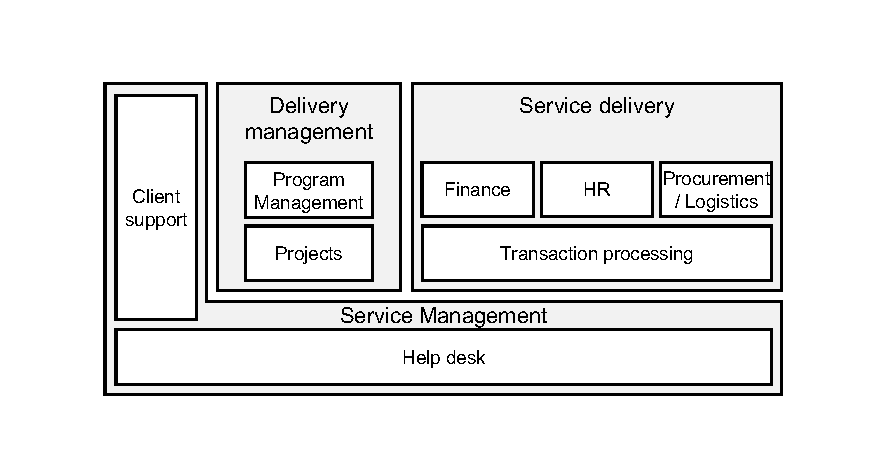
\includegraphics[width=.8\textwidth]{figures/scheweproc.pdf}\\
		\quelle{\citep[\p{98}]{schewe2007}} } 
\end{figure}
\subsection{Selected Reference Models}

\label{app:refmods}
	\begin{figure}[caption={SCOR Model}, label={fig:scor}]
	{	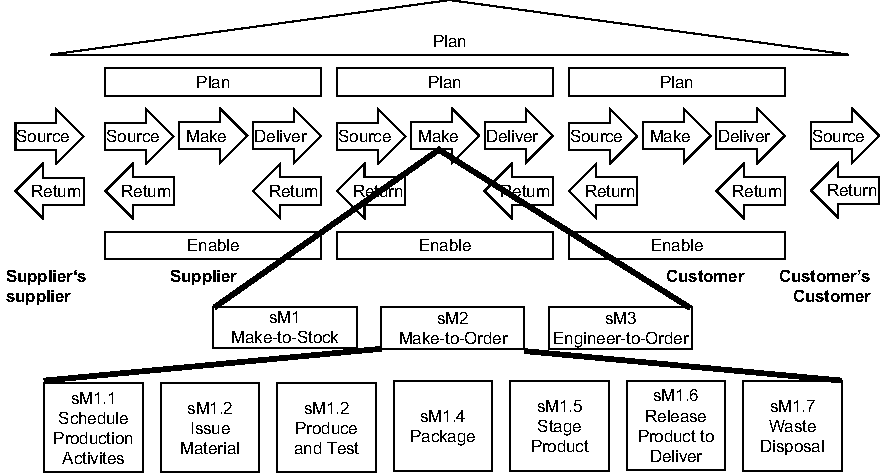
\includegraphics[width=.8\textwidth]{figures/scor.pdf}\\
	\parbox{.8\textwidth}{\quelle{\citep{APICS2015}}}} 
\end{figure}

	\begin{figure}[caption={Retail-H}, label={fig:retailh}]
	{	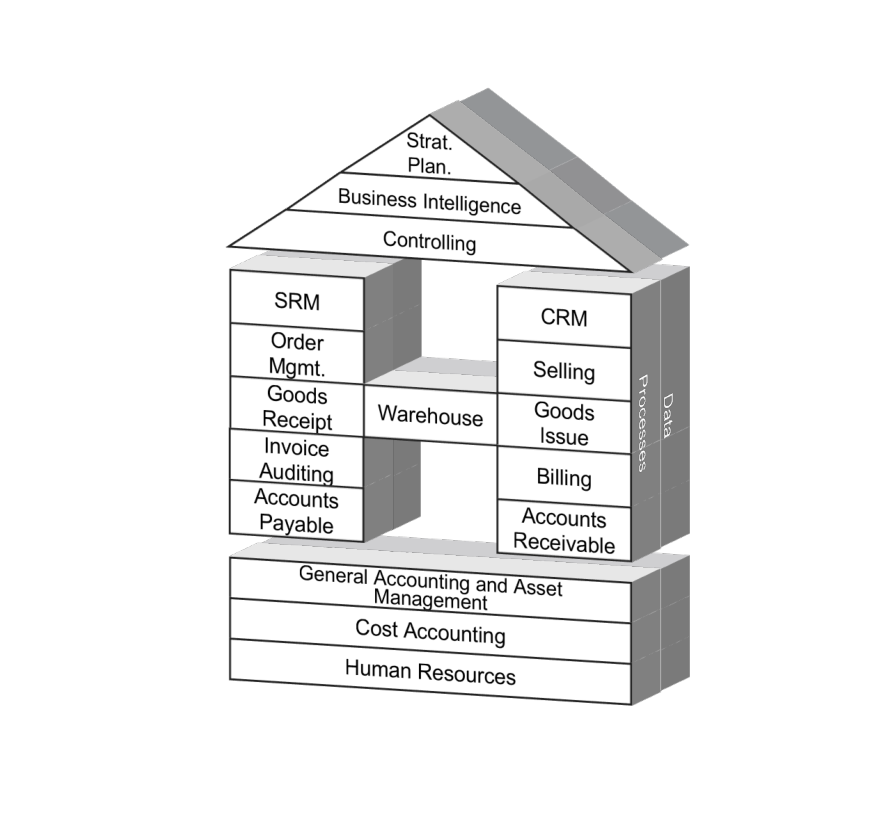
\includegraphics[width=.6\textwidth]{figures/retailh.pdf}
	\\ \parbox{0.6\textwidth}{\quelle{\citep{becker2004handelsinformationssysteme}}}}

	
\end{figure}

\subsection{icebricks Example}
\label{app:iceb}
\begin{figure}[caption={icebricks Process Structure Example: Retail-H \acrshort{CRM} Process}, label={fig:soldes}]
	\begin{subfigure}[c]{.32\textwidth}
		\begin{tikzpicture}
		[node distance=.5cm, start chain=going below,font=\sffamily]
		\node[punktchain, rounded corners=0pt, fill= gray!10, join=by {-}] (eins)      {maintain customer master data};
		\node[punktchain, rounded corners=0pt, join=by {-}] (zwei)      {maintain customer contacts};
		\node[punktchain, rounded corners=0pt, join=by {-}] (drei)      {perform goods planning};
		\node[punktchain, rounded corners=0pt, join=by {-}] (drei)      {...};
		\end{tikzpicture}
		\caption{Selection of CRM Process Components (Detail Processes)}\label{fig:retailh:main}
	\end{subfigure}
\begin{subfigure}[c]{.05\textwidth}
	\begin{tikzpicture}
	\end{tikzpicture}
\end{subfigure}
	\begin{subfigure}[c]{.45\textwidth}
		\begin{tikzpicture}
		[node distance=.5cm, start chain=going below,font=\sffamily]
		\node[punktchain, join=by {-}] (eins)      {maintain customer basic data};
		\node[punktchain,join=by {-}] (zwei)      {maintain customer views};
		\node[punktchain,  join=by {-}] (drei)      {evaluate customer roles};
		\node[punktchain,  join=by {-}] (drei)      {...};
		\end{tikzpicture}
		\caption{Selection of Maintain Customer Master Data: Process Building Blocks}\label{fig:retailh:detail}
	\end{subfigure}
	
\end{figure}

\subsection{Knowledge Management frameworks}
\label{app:knowmang}

\begin{table}[caption={Knowledge Management Framework Options}, label=tab:knowmangoptions]
	\centering
	
	\begin{tabular}{p{1cm}| p{2cm} |p{2cm}|p{3cm} | p{5cm  } }
		\textbf{Year} & \textbf{Author} & \textbf{Type} & \textbf{Decision} & \textbf{Activities} \\ \hline 
		2000          & Andersen Consulting            &      Technical Report                                      & \text{\sffamily X} URL not found         & Acquire, Create, Synthesize, Share, Use to Achieve                     \\
		1999          & Knowledge Associates            & Technical Report                                       &  \text{\sffamily X} URL not found & Acquire, Develop, Retain, Share                             \\
			1997          & Van Heijst \etal            & Paper                                          &  \checkmark & Development, Consolidation, Distribution, Combination                              \\
		1996          & Marquardt            & Book                                          &  \text{\sffamily X} Book not available & Acquisition, Creation, Transfer \& Utilization, Storage                             \\
	


	\end{tabular}
	\quelle{adapted from \citep[\pf{8}]{Rubenstein_Montano_2001}}
\end{table}
\subsection{Financial Engineering in the Outsourcing Deal}
\label{app:fineng}
	\begin{figure}[caption={Financial Engineering in the Outsourcing Deal}, label={fig:scheweproc}]
	{	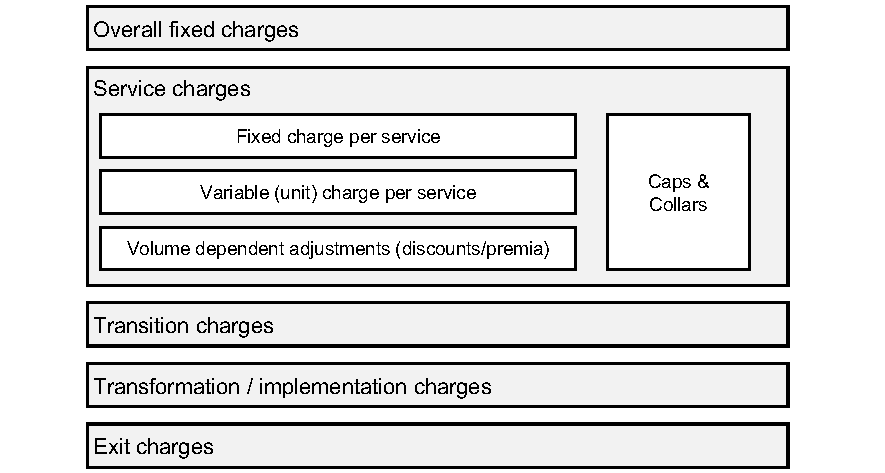
\includegraphics[width=.8\textwidth]{figures/financialengineering.pdf}
		
 }
 \parbox{.6\textwidth}{\quelle{\citep[\p{32}]{deloittehandbook}}}

\end{figure}


\subsection{Frameworks for the Product Development process}
\label{app:pdframeworks}
% Please add the following required packages to your document preamble:
% \usepackage{multirow}
\begin{table}[caption={Product Development Process Derivation}, label=tab:nsdframeworkds]
	\centering
\begin{tabular}{p{4cm}|p{5cm} |p{4.7cm}}
	\textbf{\cite{cowell1988new}} & \textbf{\cite{Edgett_1996}} adapted from \cite{cooper1988new}  & \textbf{Process in thesis}   \\ \hline \hline
	idea generation                 &                                         \\ \hline
	idea screening                  & idea screening   & evaluate idea                      \\ \hline
	& \textbullet \: preliminary market assessment     &assess market requirements    \\
	& \textbullet \: preliminary technical assessment  &assess technical requirements       \\
	& \textbullet \: detailed market study / market research \\ \hline
	concept development and testing &                       & conceptualize product                  \\ \hline
	business analysis               & business/financial analysis           & perform business analysis  \\ \hline
	\multirow{4}{*}{development}    & \textbullet \: product development      &	\multirow{4}{*}{develop product}               \\ 
	& \textbullet \: process procedures                      \\
	& \textbullet \: system design \& testing                \\
	& \textbullet \: personell training                      \\\hline
	testing                         & test market / trial sell       & test product         \\ \hline
	                      & pre-commercialization \:\:\:\:\:\:\:\:\:\:\:\:\:\:\:\:\:\:\: business analysis \\ \hline
	commercialization               & full-scale launch                   & deliver product    \\ \hline
	& post-launch review \& analysis         
\end{tabular}\\
\quelle{adapted from \citep{Edgett_1996, cowell1988new}}
\end{table}

\subsection{Some Appendix Subsection}

\lipsum[10]